\section{Objectives}
Rebuild the divider, threshold self-bias and startup-assisted references from \textit{AIC Lab.pdf}, PDF pages 22--30, and examine supply and temperature sensitivity. The model library is supplied separately by the user. The 1.0 V supply is a teaching adaptation, not a certification of the model voltage rating. Numerical plots for the handout's original 3.3 V process are not used directly as pass thresholds. The circuits are rebuilt from the handout topology; the earlier code is used only to review dimensions and omissions.

\section{Specification Mapping}
S denotes actual simulation under stated adapted conditions; D denotes analytical discussion; L denotes a numerical or validation limitation. D01 etc. identify filename prefixes.
\small\begin{longtable}{p{.46\linewidth}p{.30\linewidth}p{.15\linewidth}}\toprule
Requirement and PDF pages & Deck / check & Status \\ \midrule\endhead
Two-MOS divider and analytical comparison (22--23) & D01; DC, line AC & S+D \\
Three-MOS dual references, sizing, isolated well (24) & D02; three sizes & S+D \\
Threshold self-bias, branch conditions, zero-current solution (25) & D03; two R values & S+D \\
Startup function and injection (26--27) & D04; ramp and disconnect & S+D \\
Current setting, self-bias and complete Vbias (27--29) & D05--06; DC/AC/transient & S+D \\
Process compensation and temperature design (30) & D05--06; -20/27/85 C & S+D/L \\
Old 0.8/2.1 V and about 1.62 V examples (24,29) & 1 V adaptation & L \\
\bottomrule\end{longtable}\normalsize


\section{Circuit and Design Derivation}
\[
\beta_n(V_{ref}-V_{Tn})^2=\beta_p(V_{DD}-V_{ref}-|V_{Tp}|)^2,
\quad
V_{ref}\simeq\frac{V_{DD}-|V_{Tp}|+\sqrt{\beta_n/\beta_p}V_{Tn}}{1+\sqrt{\beta_n/\beta_p}}.
\]
\[
I_{threshold}=\frac{V_{GS1}}{R},\qquad
I_{bias}\simeq\frac{2}{\beta R_b^2}\left(1-\frac{1}{\sqrt K}\right)^2,
\qquad V_{bias}=\left(1+\frac{R_3}{R_4}\right)V_{GSn}-|V_{SGp}|.
\]These are strong-inversion, long-channel approximations for matched branches. $\beta$ must belong to the device polarity in the actual resistor-degenerated branch. The $\mu_n$ printed on PDF page 27 cannot be inserted directly into the PMOS branch of page 28; $K$ here is the corresponding PMOS geometry ratio. Body effect, finite output conductance and leakage remain in the supplied model. Old-process constants are not transplanted into the numerical results.

D01 retains $W_n/W_p/L=21/10/0.3\,\mu$m and corrects the grounded PMOS bulk. Separate cases use $W_p=20\,\mu$m or $W_n=42\,\mu$m. D02 retains two $20/0.3\,\mu$m PMOS devices and a $17.5/0.3\,\mu$m NMOS, then doubles either PMOS or NMOS widths. The middle PMOS body-source tie requires an isolated N-well in layout, with its area and isolation rules.

D03 restores the omitted M5 mirror branch, uses $R=5/10$ k$\Omega$, and holds the output at 0.5 V. M2's NMOS bulk is grounded, retaining body effect; a body-source tie would require confirmed well isolation. \texttt{.nodeset} is a solver starting hint, not hardware startup.

D04--06 implement MS1--MS3 and the four-MOS core. The old supply sine starting at 1 V is replaced by a PWL rise from zero. The complete circuit uses $R_b=1$ k$\Omega$ and $R_3/R_4=5/1$ k$\Omega$; D05 also tests $R_3=3$ k$\Omega$ and $R_b=2$ k$\Omega$.

\section{Simulation Setup}
Runs use PrimeSim HSPICE S-2021.09 win64, a baseline temperature of 27 $^\circ$C, \texttt{runlvl=5}, \texttt{accurate}, and \texttt{.op/.print/.measure} outputs. Every \texttt{.alter} resets all baseline parameters and temperature to prevent state from carrying into the next case. Actual runs completed without an error or failed measurement. Suppressed model warnings remain, so a warning-free run is not claimed. Public netlists contain no model paths. This comment marks the model setup required locally before execution; the model and its configuration remain local:
\begin{verbatim}
* MODEL_SETUP_REQUIRED
\end{verbatim}
CSV files and numerical summaries are in the lab's \texttt{results/} directory. Every figure is redrawn from actual printed data, not a waveform-viewer screenshot. \texttt{manifest.json} supplies specification mapping and case definitions.This lab contains six decks and 22 cases. D01--03 sweep supply voltage and measure the 1 Hz supply-to-output gain. D04 uses 1/30 $\mu$s ramps and a 50 $\mu$s window. D06 observes 100 $\mu$s with a 20 ns maximum step and UIC zero-charge initialization. The reported $t_{1\%}$ starts when the supply ramp begins and requires every later sample to remain within 1\% of the final value. This is a report-defined criterion, not a handout guarantee.

\section{Results and Specification Checks}
\begin{center}\small\begin{tabular}{lrrrr}\toprule
Case & $V_{ref1}$ (V) & $V_{ref2}$ (V) & $dV_o/dV_{DD}$ & $P_b$ ($\mu$W) \\ \midrule
D01/C0 & 0.403 & -- & 0.273 & 99.87 \\
D01/C1 & 0.432 & -- & 0.316 & 163.03 \\
D01/C2 & 0.375 & -- & 0.239 & 119.20 \\
D02/C0 & 0.300 & 0.650 & -- & -- \\
D02/C1 & 0.322 & 0.661 & -- & -- \\
D02/C2 & 0.278 & 0.639 & -- & -- \\
\bottomrule\end{tabular}\end{center}

\begin{figure}[htbp]\centering
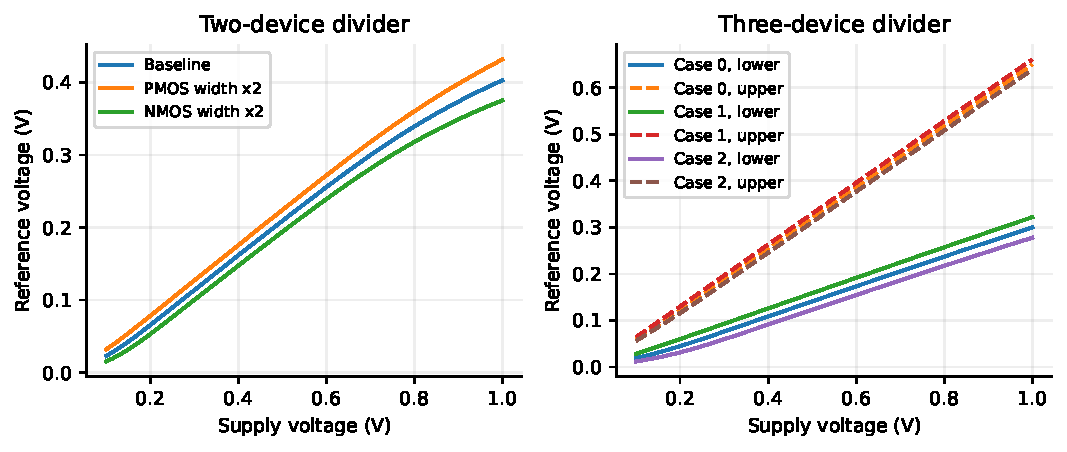
\includegraphics[width=\linewidth]{figures/reference_dividers.pdf}
\caption{Actual supply sweeps of both divider references. The old 2.1 V upper reference is unattainable with the present 1 V supply.}
\end{figure}
\begin{center}\small\begin{tabular}{lrrrr}\toprule
Case & Temp. ($^\circ$C) & $V_{ref}$ (V) & $I_{DD}$ ($\mu$A) & $|A_{supply}|$ \\ \midrule
D05/C0 & 27 & 0.44410 & 311.95 & 0.01283 \\
D05/C1 & -20 & 0.37291 & 278.86 & 3.02680 \\
D05/C2 & 85 & 0.61066 & 420.07 & 0.47272 \\
D05/C3 & 27 & 0.21186 & 313.62 & 0.05349 \\
D05/C4 & 27 & 0.22662 & 203.08 & 1.97827 \\
\bottomrule\end{tabular}\end{center}
\begin{center}\small\begin{tabular}{lrrrr}\toprule
Case & Ramp ($\mu$s) & $V_{final}$ (V) & $t_{1\%}$ ($\mu$s) & $P_b$ ($\mu$W) \\ \midrule
D06/C0 & 1 & 0.44408 & 4.18 & 311.94 \\
D06/C1 & 30 & 0.44410 & 27.82 & 311.95 \\
D06/C2 & 1 & 0.37291 & 12.72 & 278.86 \\
D06/C3 & 1 & 0.61066 & 1.80 & 420.07 \\
D06/C4 & 1 & 0.44404 & 4.18 & 311.92 \\
\bottomrule\end{tabular}\end{center}
\begin{center}\small\begin{tabular}{lrrr}\toprule
Case & $I_{inj,pk}$ (nA) & $I_{inj,final}$ (nA) & $I_{core}$ ($\mu$A) \\ \midrule
D04/C0 & 222.739 & 3.8605 & 103.102 \\
D04/C1 & 3.978 & 3.8009 & 103.098 \\
D04/C2 & 0.087 & 0.0000 & 103.089 \\
D04/C3 & 0.023 & 0.0000 & 103.090 \\
\bottomrule\end{tabular}\end{center}
D01 follows the analytical trend: stronger relative PMOS drive raises the output; stronger NMOS drive lowers it. D03 at 5 k$\Omega$ gives $V_{ref}=0.39866$ V, so $V_{ref}/R=79.732\,\mu$A; M5 measures approximately $81.000\,\mu$A. Geometry mismatch, unequal $V_{DS}$ and body effect must be considered in that difference.

D05/C0 is baseline; C1/C2 are -20/85 $^\circ$C; C3 uses $R_3=3$ k$\Omega$; C4 uses $R_b=2$ k$\Omega$. D06/C0--C4 are baseline, slow ramp, cold, hot and disconnected startup. In D04/C2--C3 the core still starts in these nominal simulations with the injection path disconnected. This observation is retained and does not show that startup is unnecessary for every ramp and corner.
\begin{figure}[htbp]\centering
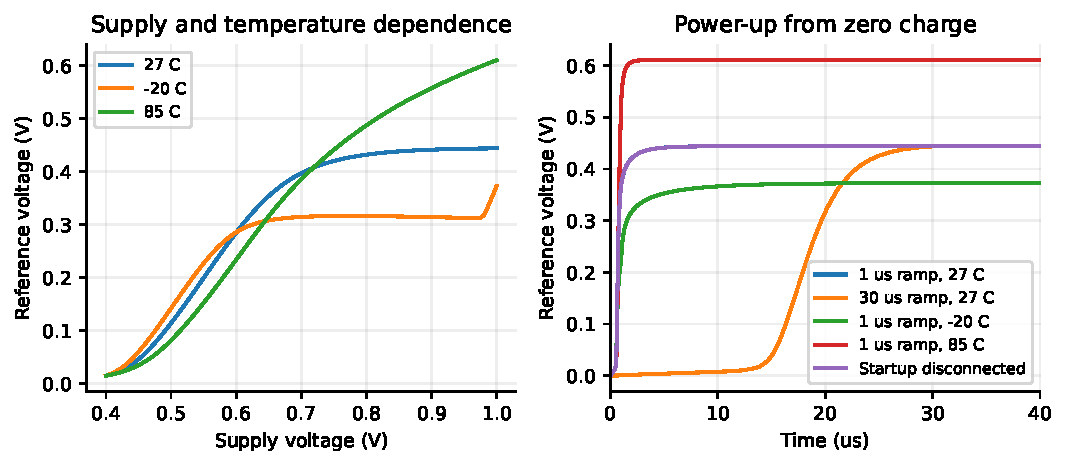
\includegraphics[width=\linewidth]{figures/reference_startup.pdf}
\caption{Complete-reference DC temperature sweeps and startup. Temperature drift and the cold DC branch transition are retained.}
\end{figure}


\section{Discussion}
Zero current is also a self-bias equilibrium. Near $I=0$, division and the strong-inversion derivation of the nonzero solution are not valid. Startup injects temporary current to leave that state and should then weaken to avoid disturbing the reference. The fast ramp gives approximately 222.7 nA peak injection and 3.86 nA at steady state. The slow ramp lacks the same spike, demonstrating ramp and trajectory dependence. Nominal startup without the injection path can result from leakage and numerical initial perturbations; it is not a cross-corner startup design.

PDF page 29 says approximately 1.62 mV while the plot is near 1.62 V. This is treated as a unit ambiguity, and neither value is imposed as a required 1 V result. Divider references depend on threshold, mobility and geometry. Resistor degeneration reduces supply dependence but retains sensitivity to $\beta$, resistance and temperature. The complete reference still drifts substantially from -20 to 85 $^\circ$C and is not fully process- or temperature-compensated. Temperature stabilization would require complementary temperature-coefficient terms, resistor selection and trimming, followed by validation with available corner and temperature models.

\section{Conclusion}
Every handout topology, startup question and compensation discussion has corresponding code and actual results. A reference near 0.444 V is obtained under the stated 1 V conditions. Original-process amplitude, complete process compensation and cross-corner startup reliability are not claimed as passed.

